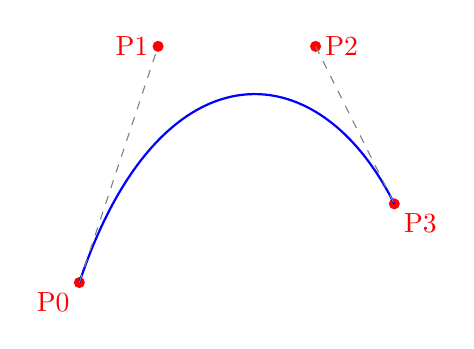
\begin{tikzpicture}
  \coordinate (A) at (0,0);
  \coordinate (B) at (1,3);
  \coordinate (C) at (3,3);
  \coordinate (D) at (4,1);
  \fill[red] (A) circle (2pt) node[below left] {P0};
  \fill[red] (B) circle (2pt) node[left] {P1};
  \fill[red] (C) circle (2pt) node[right] {P2};
  \fill[red] (D) circle (2pt) node[below right] {P3};
  \draw[thick,blue] (A) .. controls (B) and (C) .. (D);
  \draw[dashed,gray] (A) -- (B);
  \draw[dashed,gray] (C) -- (D);
\end{tikzpicture}